\documentclass[12pt]{article}
\usepackage[utf8]{inputenc}
\usepackage{graphicx}
\usepackage{amsmath}


\begin{document}

\begin{center}\textbf{Golden Ratio}\end{center}

In mathematics, two quantities are in the golden ratio if their ratio is the same as the ratio of their sum to the larger of the two quantities.The figure on the right illustrates the geometric relationship. Expressed algebraically, for quantities a and b with a $>$ b $>$ 0,
\begin{figure}[h]
    \centering
    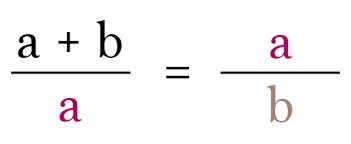
\includegraphics[scale=0.3]{download.png}
\end{figure}

The golden ratio is an irrational number represented by the Greek Symbol $\phi$ or $\varphi$. The Golden ratio is the solution to the quadratic equation $x^2-x-1=0$. with a value of,
$\varphi=$1.6180339887 . .
\par
Some of the greatest mathematical minds of all ages, from Pythagoras and Euclid in ancient Greece, through the medieval Italian mathematician Leonardo of Pisa and the Renaissance astronomer Johannes Kepler, to present-day scientific figures such as Oxford physicist Roger Penrose, have spent endless hours over this simple ratio and its properties.Golden ratio has many applications in Art,Architecture, Books,Music and Design.
Many Famous architects and artists,including Le Corbusier and Salvador Dalí, have proportioned their works to approximate the golden ratio—especially in the form of the golden rectangle, in which the ratio of the longer side to the shorter is the golden ratio—believing this proportion to be aesthetically pleasing.
It is an interesting fact that the famous Mona Lisa painted by Leonardo Da Vinci also employs the Golden ratio.
\begin{figure}[h]
    \centering
    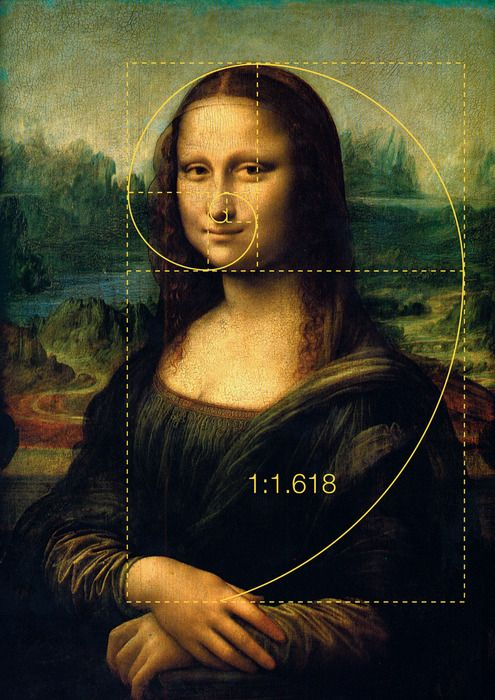
\includegraphics[scale=0.20]{text.jpg}
\end{figure}


Reference:-https://en.wikipedia.org/wiki/Golden_ratio


\end{document}